%
\documentclass[]{ctexart}
\usepackage{lmodern}
\usepackage{amssymb,amsmath}
\usepackage{ifxetex,ifluatex}
\usepackage{fixltx2e} % provides \textsubscript
\ifnum 0\ifxetex 1\fi\ifluatex 1\fi=0 % if pdftex
  \usepackage[T1]{fontenc}
  \usepackage[utf8]{inputenc}
  \usepackage{textcomp} % provides euro and other symbols
\else % if luatex or xelatex
  \usepackage{unicode-math}
  \defaultfontfeatures{Ligatures=TeX,Scale=MatchLowercase}
\fi
% use upquote if available, for straight quotes in verbatim environments
\IfFileExists{upquote.sty}{\usepackage{upquote}}{}
% use microtype if available
\IfFileExists{microtype.sty}{%
\usepackage[]{microtype}
\UseMicrotypeSet[protrusion]{basicmath} % disable protrusion for tt fonts
}{}
\IfFileExists{parskip.sty}{%
\usepackage{parskip}
}{% else
\setlength{\parindent}{0pt}
\setlength{\parskip}{6pt plus 2pt minus 1pt}
}
\usepackage{hyperref}
\hypersetup{
            pdfborder={0 0 0},
            breaklinks=true}
\urlstyle{same}  % don't use monospace font for urls
\usepackage{longtable,booktabs}
% Fix footnotes in tables (requires footnote package)
\IfFileExists{footnote.sty}{\usepackage{footnote}\makesavenoteenv{longtable}}{}
\usepackage{graphicx,grffile}
\makeatletter
\def\maxwidth{\ifdim\Gin@nat@width>\linewidth\linewidth\else\Gin@nat@width\fi}
\def\maxheight{\ifdim\Gin@nat@height>\textheight\textheight\else\Gin@nat@height\fi}
\makeatother
% Scale images if necessary, so that they will not overflow the page
% margins by default, and it is still possible to overwrite the defaults
% using explicit options in \includegraphics[width, height, ...]{}
\setkeys{Gin}{width=\maxwidth,height=\maxheight,keepaspectratio}
\setlength{\emergencystretch}{3em}  % prevent overfull lines
\providecommand{\tightlist}{%
  \setlength{\itemsep}{0pt}\setlength{\parskip}{0pt}}
\setcounter{secnumdepth}{0}
% Redefines (sub)paragraphs to behave more like sections
\ifx\paragraph\undefined\else
\let\oldparagraph\paragraph
\renewcommand{\paragraph}[1]{\oldparagraph{#1}\mbox{}}
\fi
\ifx\subparagraph\undefined\else
\let\oldsubparagraph\subparagraph
\renewcommand{\subparagraph}[1]{\oldsubparagraph{#1}\mbox{}}
\fi

% set default figure placement to htbp
\makeatletter
\def\fps@figure{htbp}
\makeatother


\date{}

\begin{document}

\hypertarget{yoom-meetings-ux5728ux7ebfux97f3ux89c6ux9891ux4f1aux8baeux7cfbux7edf-ux8f6fux4ef6ux9700ux6c42ux6587ux6863}{%
\section{Yoom Meetings 在线音视频会议系统
软件需求文档}\label{yoom-meetings-ux5728ux7ebfux97f3ux89c6ux9891ux4f1aux8baeux7cfbux7edf-ux8f6fux4ef6ux9700ux6c42ux6587ux6863}}

\begin{quote}
10185101210 陈俊潼
\end{quote}

Index

\tableofcontents

\hypertarget{ux7b80ux4ecb--introduction}{%
\subsection{简介 / Introduction}\label{ux7b80ux4ecb--introduction}}

\hypertarget{ux613fux666f--purpose}{%
\subsubsection{愿景 / Purpose}\label{ux613fux666f--purpose}}

Yoom Meetings
是一套高性能、高效、创新、安全的多人会议协作系统。后疫情时代,网上协作、远程办公成了大量中小企业的趋势,Work
From Home 的流行也让音视频会议成为了企业推进工作必不可少的环节。Yoom
Meetings 提供了一套高可用的可靠的会议系统。Yoom Meetings
支持多端入会、会中特效、字幕翻译,同时也针对企业会议室应用提供了整体解决方案,包括
Yoom 会议室的功能,兼容传统视频会议的 SIP
协议连接,支持主流视频会议品牌设备接入 Yoom
音视频会议。本音视频会议系统旨在提高远程协作的流程,提供流畅的音视频会议体验,为各体量的有音视频会议需求的企业提供可靠优质的解决方案。

Yoom Meetings 希望助力组织和个人更高效、更流畅、更满意。

\hypertarget{ux8303ux56f4--scope}{%
\subsubsection{范围 / Scope}\label{ux8303ux56f4--scope}}

Yoom Meetings
针对从数十人的小型团队到上万人的大型高校、企业都提出了安全可靠的解决方案,我们将处理音视频会议从发起、会中再到会议结束的过程中的所有过程。为了提供流畅的入会流程,提供了使用
ID 入会、链接入会和 PSTN
入会等多种解决方案;在会中为主持人和联席主持人提供了细粒度的权限管理方案和权限控制;在会后提供了详细的会议参会情况记录与聊天记录回顾,方便主持人回顾会议内容。

本系统的系统关联图如下:

\begin{figure}
\centering
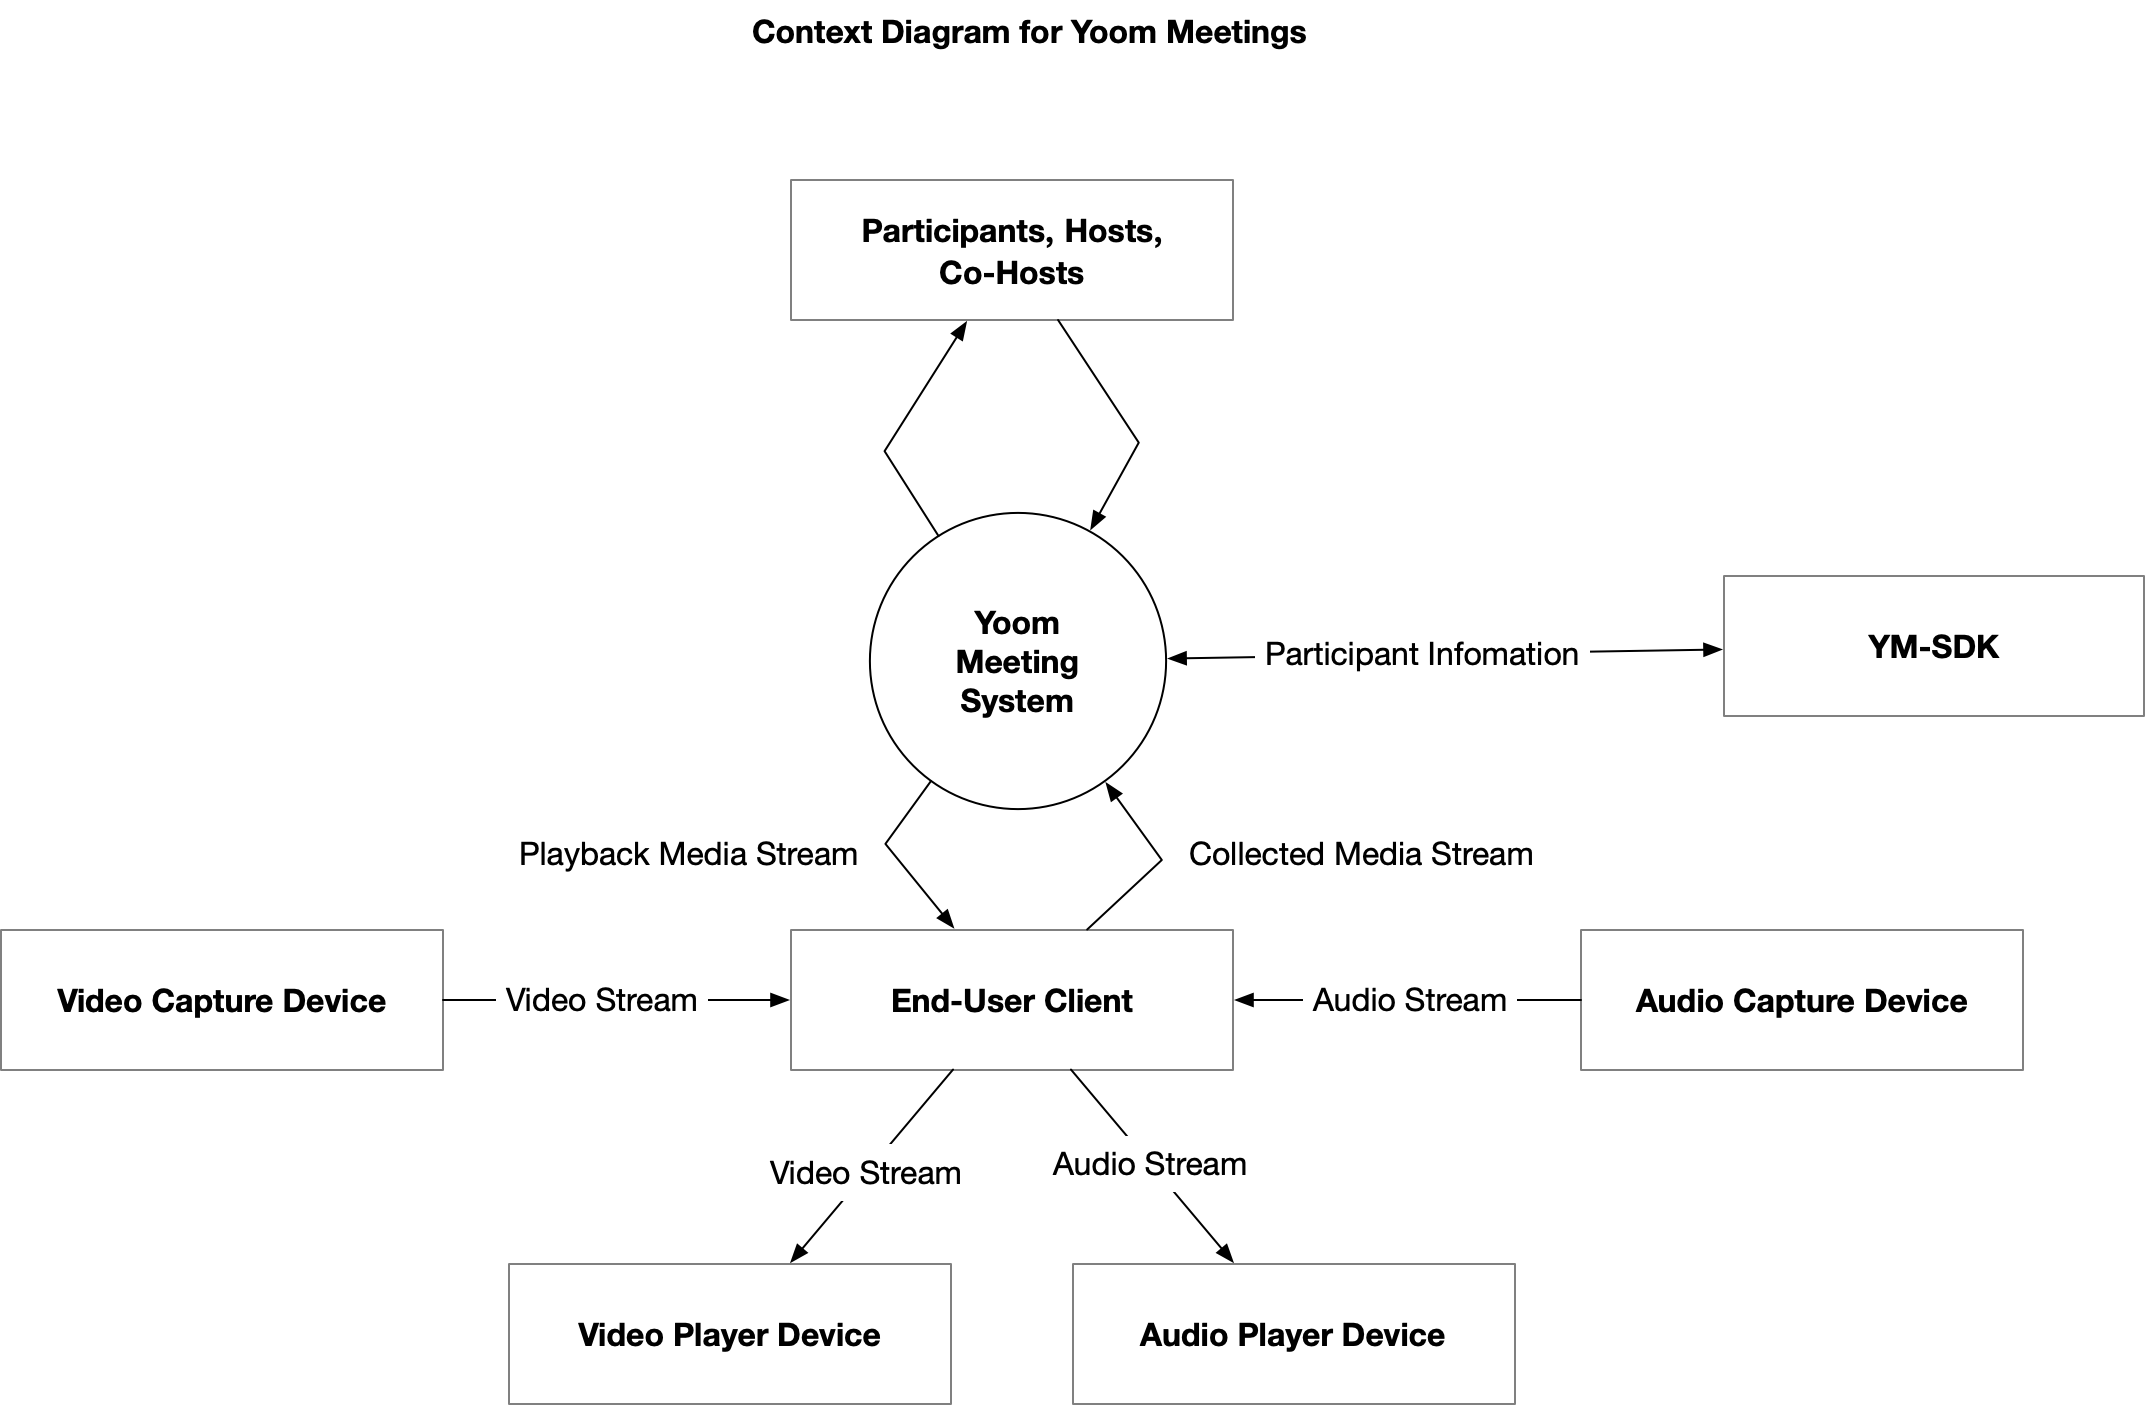
\includegraphics{/Users/billchen/Workspace/LearningRepo/Course/SoftwareRequirements/Yoom/YoomMeetings/Context Diagram.png}
\caption{}
\end{figure}

\hypertarget{ux672fux8bedux5b9aux4e49--definition}{%
\subsubsection{术语定义 /
Definition}\label{ux672fux8bedux5b9aux4e49--definition}}

\begin{longtable}[]{@{}lll@{}}
\toprule
术语 & 英文全称 & 含义\tabularnewline
\midrule
\endhead
RTC & Real Time Conference &
实时音视频,本系统提供高并发、低延迟、高清流畅、安全可靠的音视频服务。\tabularnewline
SIP & Session Initiation Protocol & 会话初始协议,由IETF(Internet
Engineering Task Force,因特网工程任务组)制定的多媒体通信协议。
它是一个基于文本的应用层控制协议,用于创建、修改和释放一个或多个参与者的会话。\tabularnewline
PSTN & Public Switched Telephone Network &
公共交换网络,使用电话号码邀请参会人拨入会议的协议\tabularnewline
VC & Video Conference & 视频会议系统\tabularnewline
PB & Protocol Buffers &
约定接口和相关数据结构的数据描述语言\tabularnewline
App Container & - & App的容器,每个独立的App都需要有一个 App Container
来实现自己的 Container,包括 apis、UI-SDK、PageManager\tabularnewline
YM-SDK & - & 包含底层 C++ 能力,视频会议所使用的 RTC SDK.\tabularnewline
YM-Core & - &
\vtop{\hbox{\strut 包视频会议的核心业务逻辑,会被多个App复用。运行于App
Container内。包括:}\hbox{\strut - UI-SDK:包含 UI 部分的外部 SDK
封装}\hbox{\strut - 状态机:视频会议所使用的状态机}\hbox{\strut -
Page-Manager:界面管理及界面容器}}\tabularnewline
\bottomrule
\end{longtable}

\hypertarget{ux89d2ux8272ux5b9aux4e49--actors}{%
\subsubsection{角色定义 /
Actors}\label{ux89d2ux8272ux5b9aux4e49--actors}}

系统中的角色主要区分成了以下四类:

\begin{longtable}[]{lp{3cm}p{6cm}}
\toprule
角色名称 & 职责描述\tabularnewline
\midrule
\endhead
Host &
会议主持人,具备结束会议、管理成员、转移主持人权限、终止会议、禁音所有参会者、修改入会权限或取消禁音所有参会者等最高权限,主持人只能有一人\tabularnewline
Co-Host &
联席主持人,联席主持人可以具有多人,具备主持人除转移主持人以外的所有权限,协助管理会议状态和入会这信息\tabularnewline
Participant &
会议的参与者,可以控制自己的会议状态和离开会议,无法对其他人的状态做出修改或终止本会议\tabularnewline
Non-Participant & 会议的非参与者,指准备加入会议的用户,可以通过
PSTN、会议
ID、会议链接加入会议。包括未进入会议室的用户和在会议室等候(如需要)的用户。\tabularnewline
\bottomrule
\end{longtable}

\hypertarget{ux6982ux89c8--overview}{%
\subsubsection{概览 / Overview}\label{ux6982ux89c8--overview}}

\hypertarget{ux72b6ux6001ux673a}{%
\paragraph{状态机}\label{ux72b6ux6001ux673a}}

Yoom 对每个参会者维持了一个状态机,用户指示当前用户的状态。

\texttt{YMCORE-STATEMACHINE}:状态机图

\begin{figure}
\centering
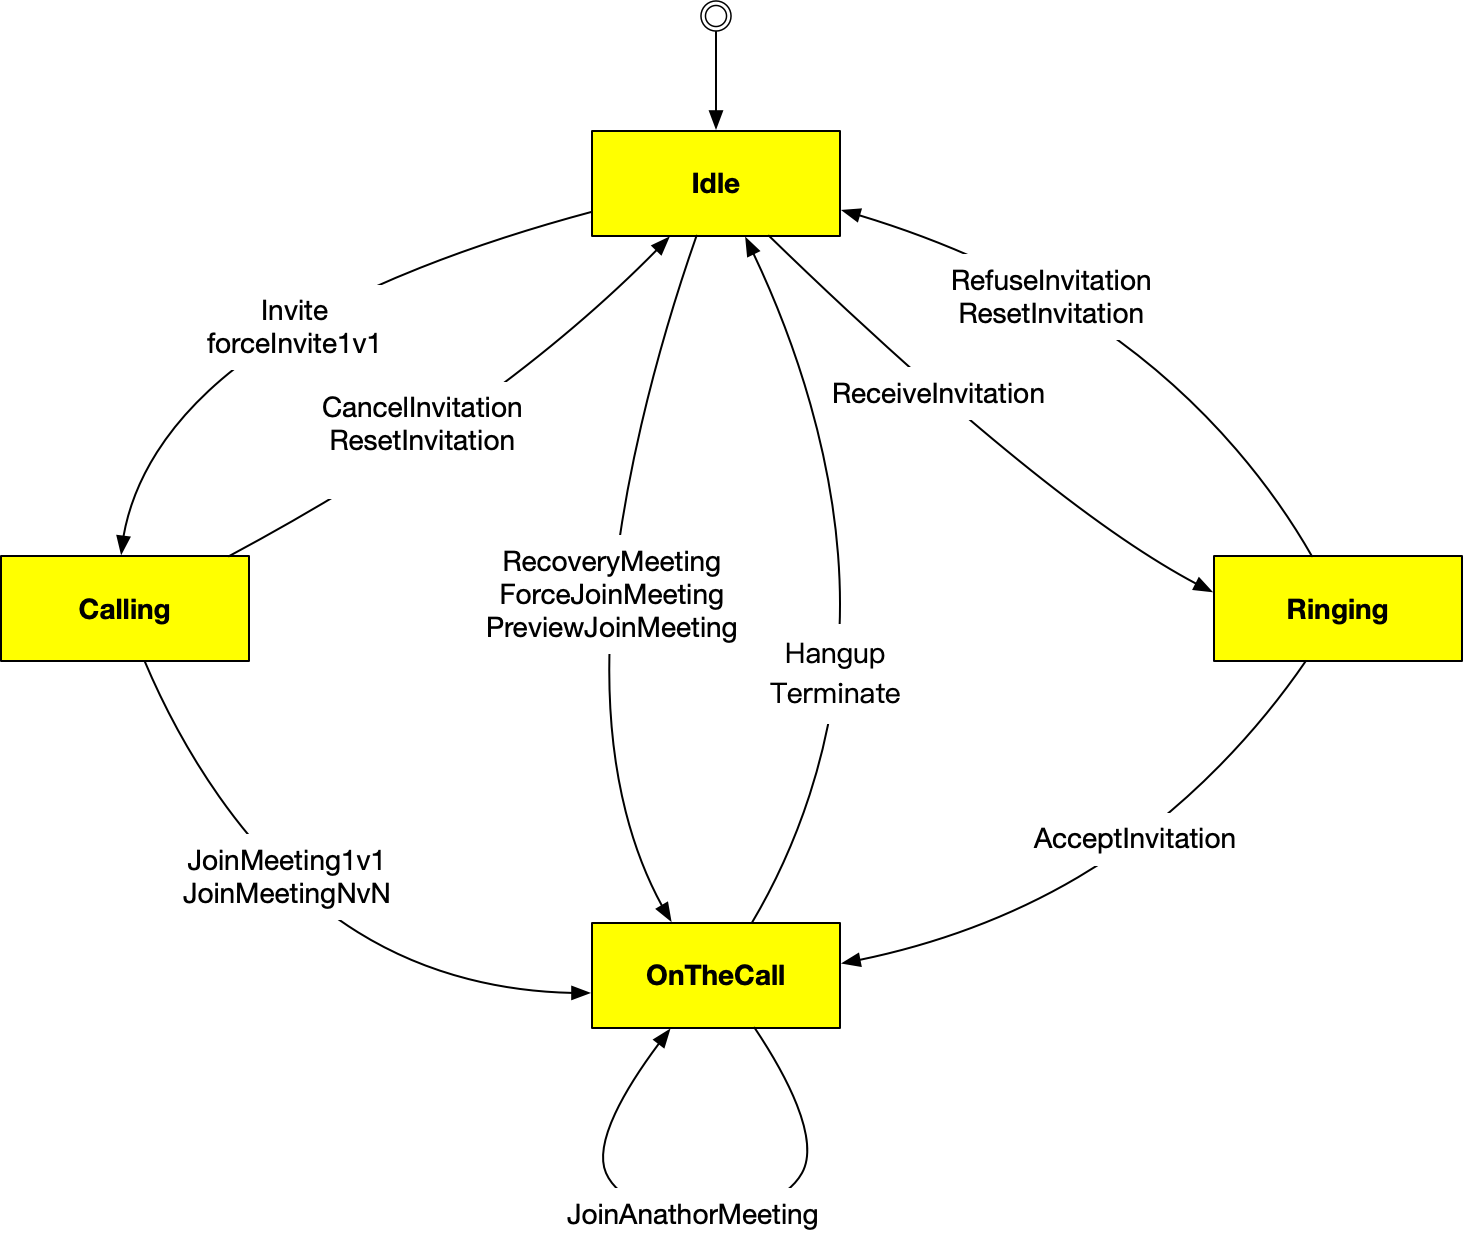
\includegraphics{/Users/billchen/Workspace/LearningRepo/Course/SoftwareRequirements/Yoom/YoomMeetings/State Machine.png}
\caption{}
\end{figure}

各状态含义如下:

\begin{longtable}[]{@{}ll@{}}
\toprule
State & 含义\tabularnewline
\midrule
\endhead
IDLE & 空闲状态,未进入会议的待命状态\tabularnewline
CALLING & 当用户\textbf{呼叫}其他用户时,弹出的呼叫页面\tabularnewline
RINGING & 当用户\textbf{被叫}时,弹出的被叫页面\tabularnewline
ONTHECALL & 处在会议中的状态\tabularnewline
\bottomrule
\end{longtable}

\hypertarget{ux72b6ux6001ux8fc1ux79fbux63a5ux53e3}{%
\paragraph{状态迁移接口}\label{ux72b6ux6001ux8fc1ux79fbux63a5ux53e3}}

\begin{itemize}
\item
  \texttt{invite} 正常情况下的1v1会议或多人会议的邀请操作
\item
  \texttt{joinMeeting}正常情况下

  \begin{itemize}
  \item
    1v1会议:在服务端创建会议成功,并且对方接听,然后进入ON\_THE\_CALL
  \item
    多人会议:在服务端创建会议成功,然后进入ON\_THE\_CALL
  \end{itemize}
\item
  \texttt{cancelInvitation}取消1v1会议邀请
\item
  \texttt{receiveInvitation} 收到邀请,进入Ringing状态
\item
  \texttt{refuseInvitation} Ringing状态拒绝邀请
\item
  \texttt{resetInvitation}

  \begin{itemize}
  \item
    CALLING状态下:重置会议1v1会议或多人会议的邀请,一般用于创建会议失败等等意外情况
  \item
    RINGING状态下:重置会议1v1会议或多人会议的邀请,一般用于创建会议失败等等意外情况
  \end{itemize}
\item
  \texttt{acceptInvitation}
  用户点击操作接受按钮,接受邀请并进入ON\_THE\_CALL
\item
  \texttt{forceAcceptInvitation}
  用户先收到了Zoom多人会议的RINGING推送,然后通过卡片加入相同会议
\item
  \texttt{forceInvite1v1}
  跨设备切换到1v1会议,具体情况是:别的设备在会中,本设备发起1v1会议。会先弹出确认框,确认后后端直接下发状态然后进入CALLING状态
\item
  \texttt{recoveryMeeting}
  客户端整体意外crash并重启之后,会自动恢复多人会议
\item
  \texttt{forceJoinMeeting} 通过卡片进入Zoom多人会议,并加入会议的操作
\item
  \texttt{previewJoinMeeting}
  通过卡片进入自研SDK的Lark多人会议,打开预览界面,然后点击加入会议的操作
\item
  \texttt{hangup}

  \begin{itemize}
  \item
    主动挂断会议(结束会议 / 自己离开会议)
  \item
    SDK 报错或者加入会议失败导致了离开会议
  \item
    当参会者申请加入另一个会议时,强制离开当前会议
  \end{itemize}
\item
  \texttt{terminate}

  \begin{itemize}
  \item
    被踢出会议
  \item
    1v1会议对方断线或离开
  \item
    其他情况下,服务端下发了IDLE状态会自动退出会议
  \end{itemize}
\item
  \texttt{rejoin}

  \begin{itemize}
  \item
    在 sdk 重连失败后,用户点击重新加会,调用 \texttt{rejoinVideoChat}
    来重新进入会议
  \end{itemize}
\end{itemize}

\hypertarget{ux4e1aux52a1ux9700ux6c42--solutions}{%
\subsection{业务需求 /
Solutions}\label{ux4e1aux52a1ux9700ux6c42--solutions}}

系统用例图如下图所示:

\begin{figure}
\centering
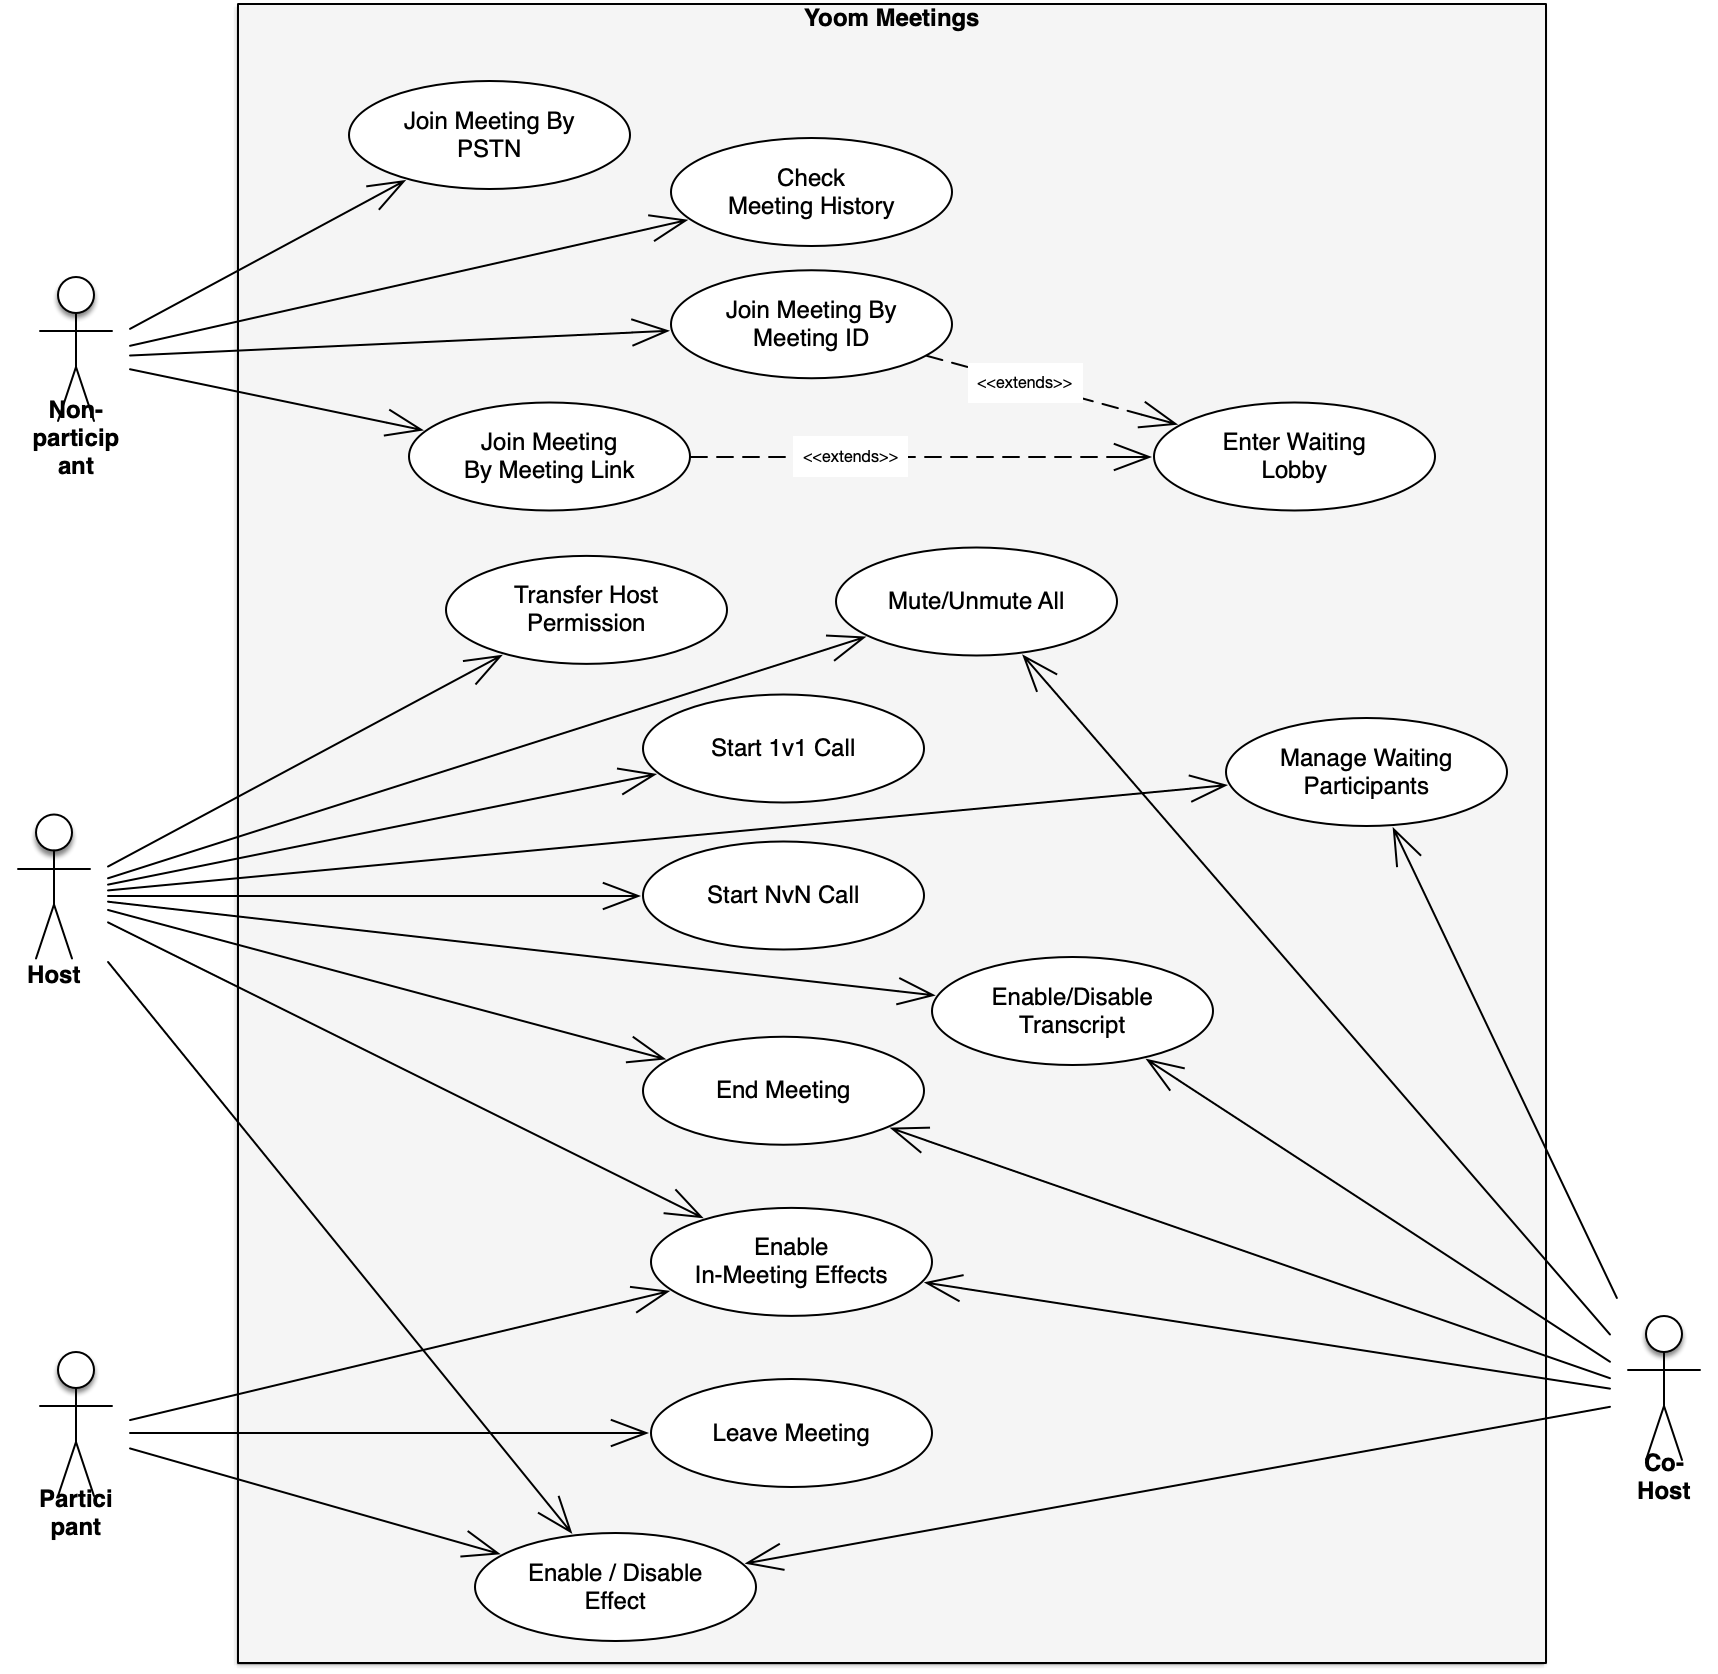
\includegraphics{/Users/billchen/Workspace/LearningRepo/Course/SoftwareRequirements/Yoom/YoomMeetings/Use Case Diagram.png}
\caption{}
\end{figure}

\hypertarget{ym10011v1-ux901aux8bdd-1}{%
\subsubsection{YM1001:1v1 通话}\label{ym10011v1-ux901aux8bdd-1}}

\hypertarget{ux7528ux6237ux754cux9762-1}{%
\paragraph{用户界面}\label{ux7528ux6237ux754cux9762-1}}

\hypertarget{ux65f6ux5e8fux56fe-1}{%
\paragraph{时序图}\label{ux65f6ux5e8fux56fe-1}}

\texttt{YM1001-SQ00:\ 1v1\_start\_invitation}:发起 1v1 邀请

\begin{figure}
\centering
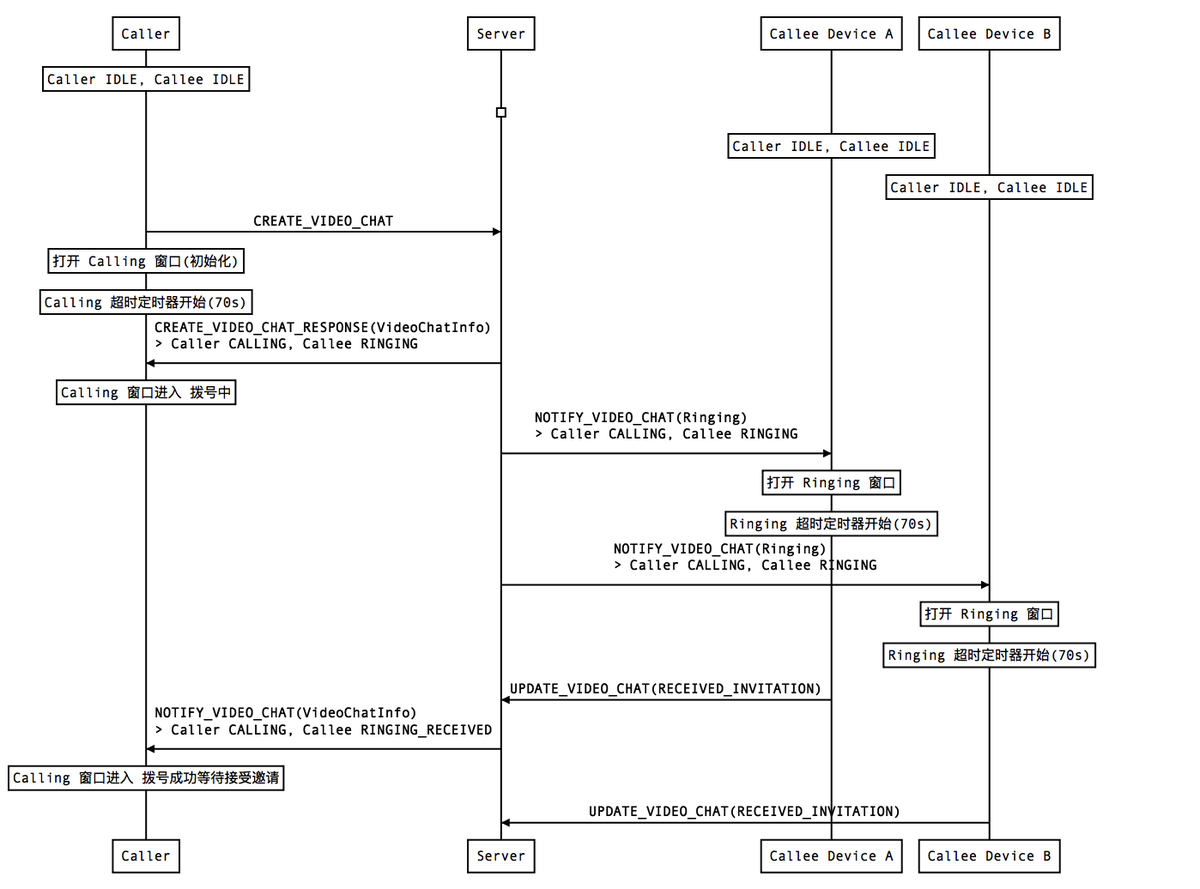
\includegraphics{/Users/billchen/Workspace/LearningRepo/Course/SoftwareRequirements/Yoom/Sequence Diagram/00_1v1_start_invitation.png}
\caption{}
\end{figure}

\texttt{YM1001-SQ01:\ 1v1\_invitation\_fail}:1v1 邀请失败:

\begin{figure}
\centering
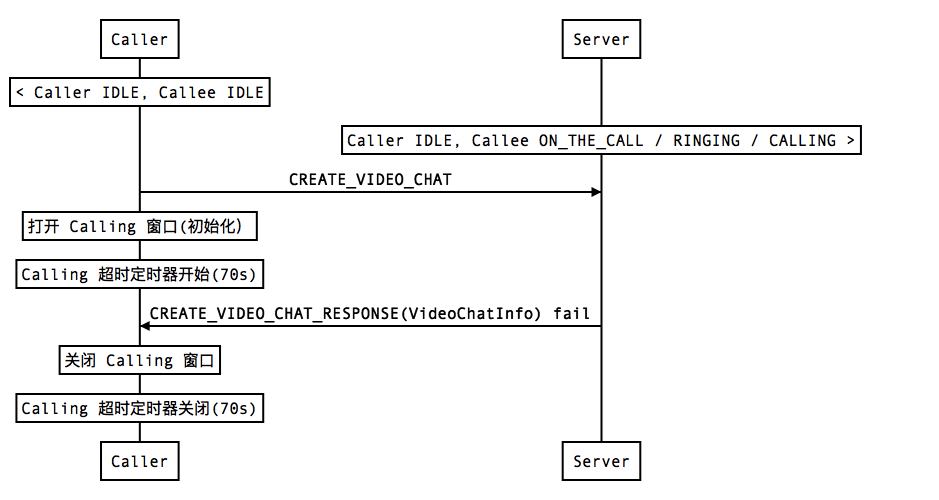
\includegraphics{/Users/billchen/Workspace/LearningRepo/Course/SoftwareRequirements/Yoom/Sequence Diagram/01_1v1_invitation_fail.png}
\caption{}
\end{figure}

\texttt{YM1001-SQ02:\ 1v1\_accept\_invitation}:1v1 通话接受邀请:

\begin{figure}
\centering
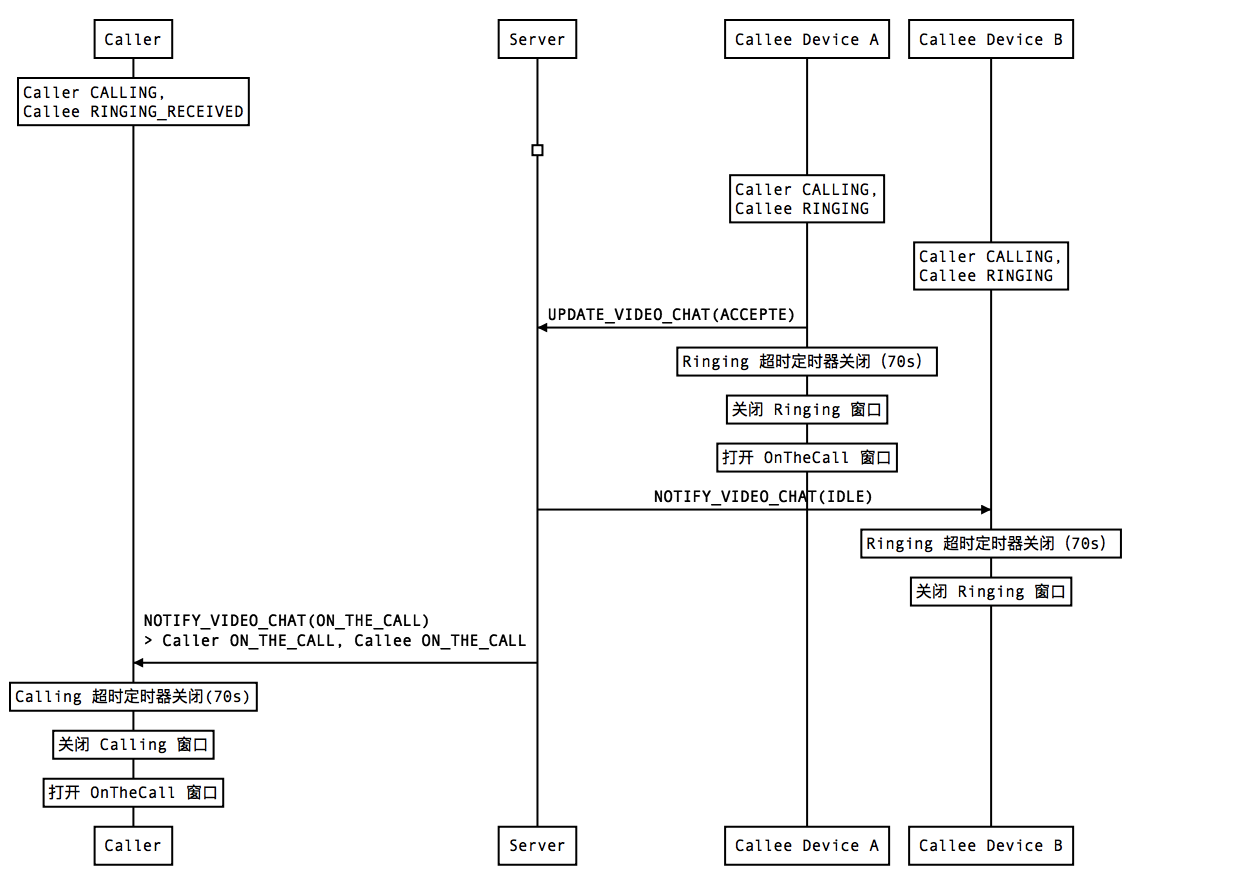
\includegraphics{/Users/billchen/Workspace/LearningRepo/Course/SoftwareRequirements/Yoom/Sequence Diagram/02_1v1_accept_invitation.png}
\caption{}
\end{figure}

\texttt{YM1001-SQ03:\ 1v1\_cancel\_invitation}:1v1 通话取消发起邀请:

\begin{figure}
\centering
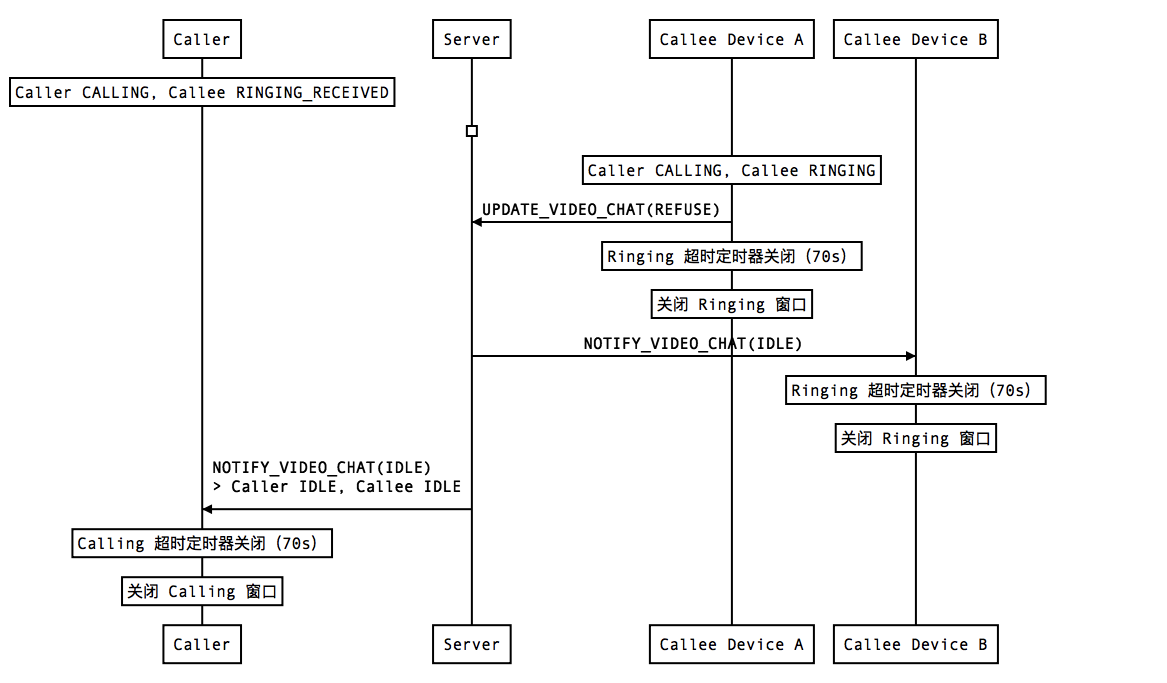
\includegraphics{/Users/billchen/Workspace/LearningRepo/Course/SoftwareRequirements/Yoom/Sequence Diagram/03_1v1_cancel_invitation.png}
\caption{}
\end{figure}

\texttt{YM1001-SQ04:\ 1v1\_hang\_over}:1v1 通话挂断(任意一方):

\begin{figure}
\centering
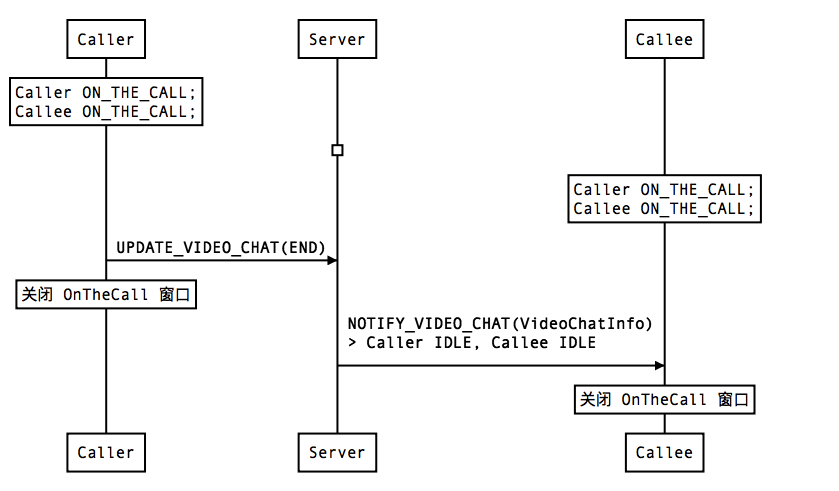
\includegraphics{/Users/billchen/Workspace/LearningRepo/Course/SoftwareRequirements/Yoom/Sequence Diagram/04_1v1_hang_over.png}
\caption{}
\end{figure}

\hypertarget{ux9700ux6c42ux63cfux8ff0ux53caux7528ux4f8bux63cfux8ff0-1}{%
\paragraph{需求描述及用例描述}\label{ux9700ux6c42ux63cfux8ff0ux53caux7528ux4f8bux63cfux8ff0-1}}

\begin{itemize}
\item
  不同用户之间应当能直接向对方发起 1v1 通话
\item
  可以使用对方的用户名、邮箱、手机号来发起 1v1 通话
\item
  非参会者可以使用
\end{itemize}

该需求涉及到的用例主要有 Join Meeting By PSTN,Join By 1v1 Invitation

\hypertarget{ux7528ux4f8bux63cfux8ff0join-meeting-by-pstn}{%
\subparagraph{用例描述:Join Meeting By
PSTN}\label{ux7528ux4f8bux63cfux8ff0join-meeting-by-pstn}}

\begin{longtable}[]{@{}ll@{}}
\toprule
Key & Value\tabularnewline
\midrule
\endhead
Use Case & Join Meeting By PSTN\tabularnewline
Actors & Non-participant, Host\tabularnewline
Pre-condition &
\vtop{\hbox{\strut 用户应当正确登录进了系统;}\hbox{\strut 用户应当被
Host 通过 PSTN 邀请通过电话拨入会议;}}\tabularnewline
Post-condition & Non-participant 被 Host 邀请进该会议\tabularnewline
Main Flow & \vtop{\hbox{\strut Non-participant
收到电话邀请}\hbox{\strut Non-participant
接受电话邀请,进入会议}}\tabularnewline
Alternative Flow & \vtop{\hbox{\strut Non-participant
当前正在另一个会议,收到电话邀请}\hbox{\strut Non-participant
选择是否接受会议邀请,如果接受邀请,则退出当前会议,并加入新的会议}\hbox{\strut 如果拒接邀请,则忽略该邀请,用户继续在原会议进行通话}}\tabularnewline
Exception & None\tabularnewline
\bottomrule
\end{longtable}

\hypertarget{ux7528ux4f8bux63cfux8ff0join-meeting-by-1v1-invitation}{%
\subparagraph{用例描述:Join Meeting By 1v1
Invitation}\label{ux7528ux4f8bux63cfux8ff0join-meeting-by-1v1-invitation}}

\begin{longtable}[]{@{}ll@{}}
\toprule
Key & Value\tabularnewline
\midrule
\endhead
Use Case & Join Meeting By Link\tabularnewline
Actors & Non-participant, Host\tabularnewline
Pre-condition &
\vtop{\hbox{\strut 用户应当正确登录进了系统;}\hbox{\strut Non-participant
拥有了 1v1 通话的邀请链接}}\tabularnewline
Post-condition & Non-participant 被 Host 邀请进该会议\tabularnewline
Main Flow & Non-participant 打开链接,进入会议\tabularnewline
Alternative Flow & \vtop{\hbox{\strut Non-participant
当前正在另一个会议,并打开了链接:}\hbox{\strut Non-participant
选择是否接受会议邀请,如果接受邀请,则退出当前会议,并加入新的会议}\hbox{\strut 如果拒接邀请,则忽略该邀请,用户继续在原会议进行通话}\hbox{\strut 该会议设置了入会权限,需要在等候室确认主持人进入会议系统之后再}}\tabularnewline
Exception & None\tabularnewline
\bottomrule
\end{longtable}

\hypertarget{ym1002nvn-ux901aux8bdd-1}{%
\subsubsection{YM1002:NvN 通话}\label{ym1002nvn-ux901aux8bdd-1}}

\hypertarget{ux7528ux6237ux754cux9762-2}{%
\paragraph{用户界面}\label{ux7528ux6237ux754cux9762-2}}

\hypertarget{ux65f6ux5e8fux56fe-2}{%
\paragraph{时序图}\label{ux65f6ux5e8fux56fe-2}}

\texttt{YM1002-SQ01:\ nvn\_start\_invitation}:NvN 通话发起邀请:

\begin{figure}
\centering
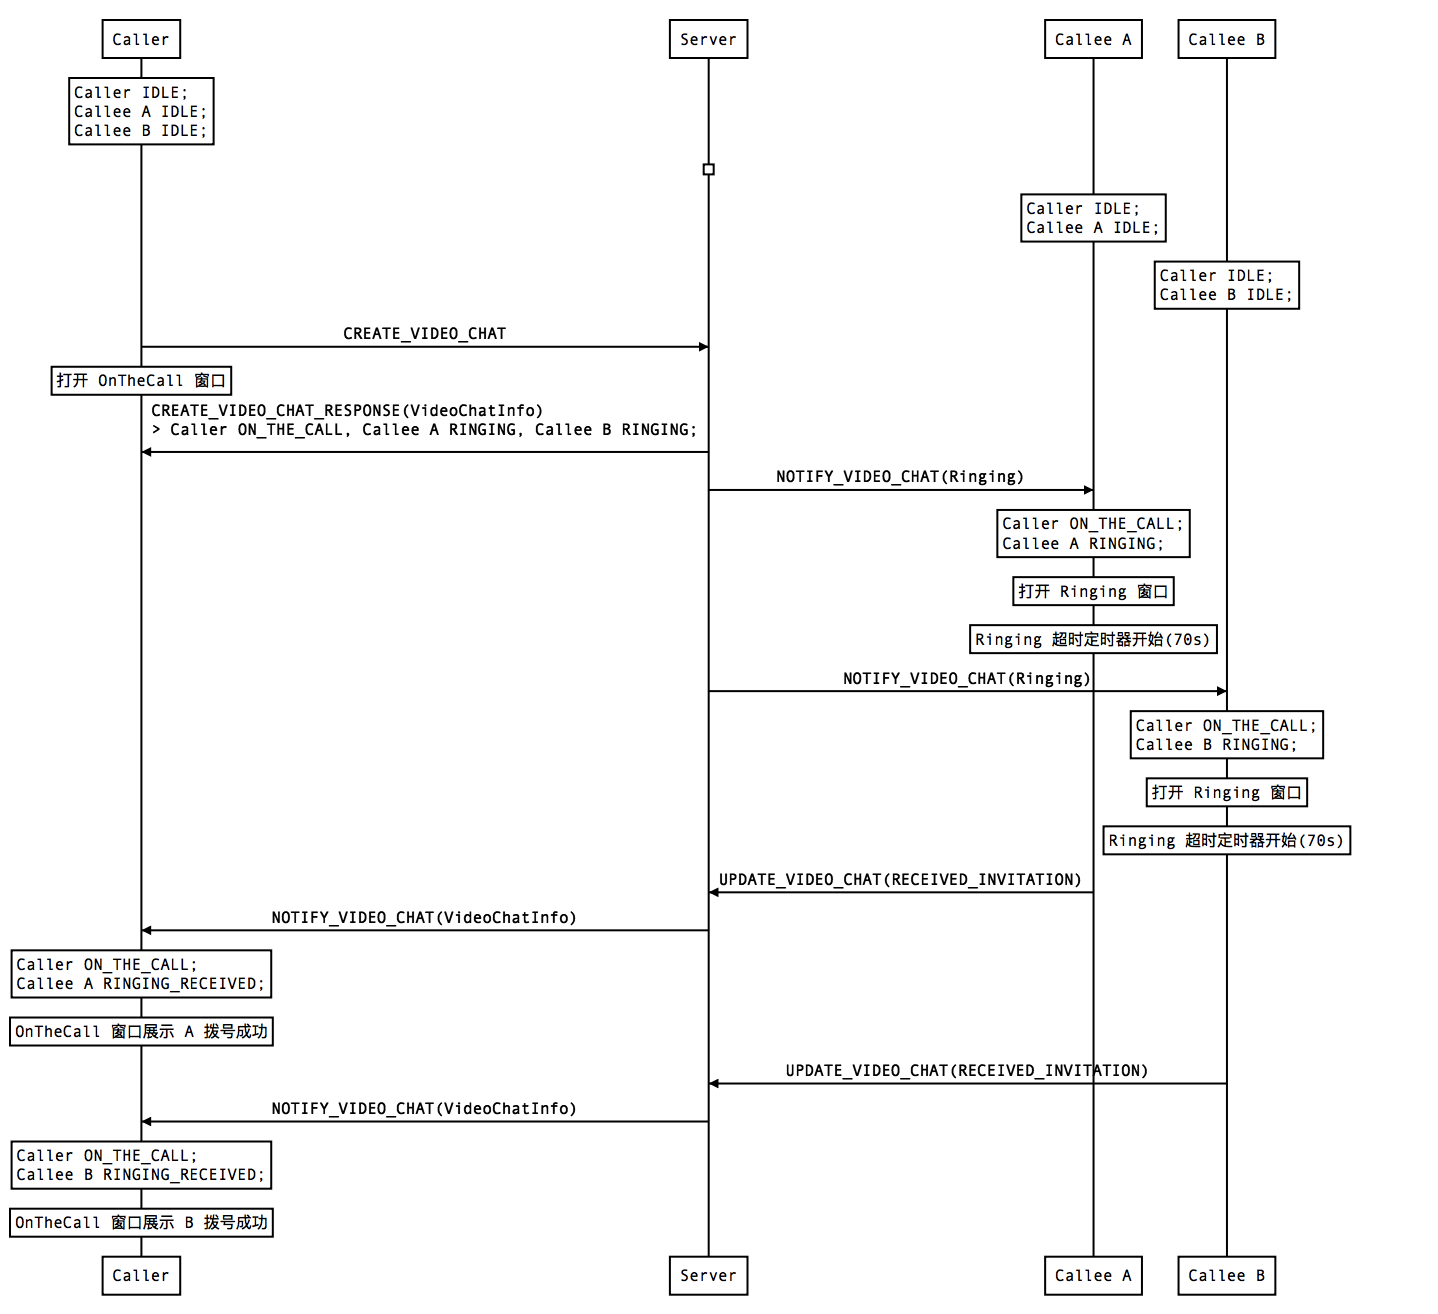
\includegraphics{/Users/billchen/Workspace/LearningRepo/Course/SoftwareRequirements/Yoom/Sequence Diagram/05_nvn_start_invitation.png}
\caption{}
\end{figure}

\texttt{YM1002-SQ02:\ nvn\_invitation\_fail}:NvN 通话邀请失败:

\begin{figure}
\centering
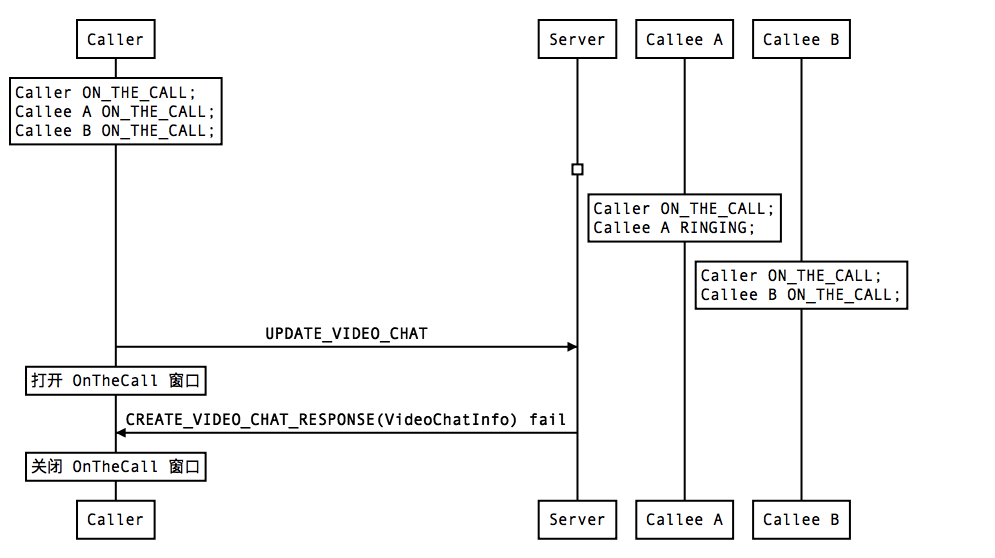
\includegraphics{/Users/billchen/Workspace/LearningRepo/Course/SoftwareRequirements/Yoom/Sequence Diagram/06_nvn_invitation_fail.png}
\caption{}
\end{figure}

\texttt{YM1002-SQ03:\ nvn\_accept\_invitation}:NvN 通话接受邀请:

\begin{figure}
\centering
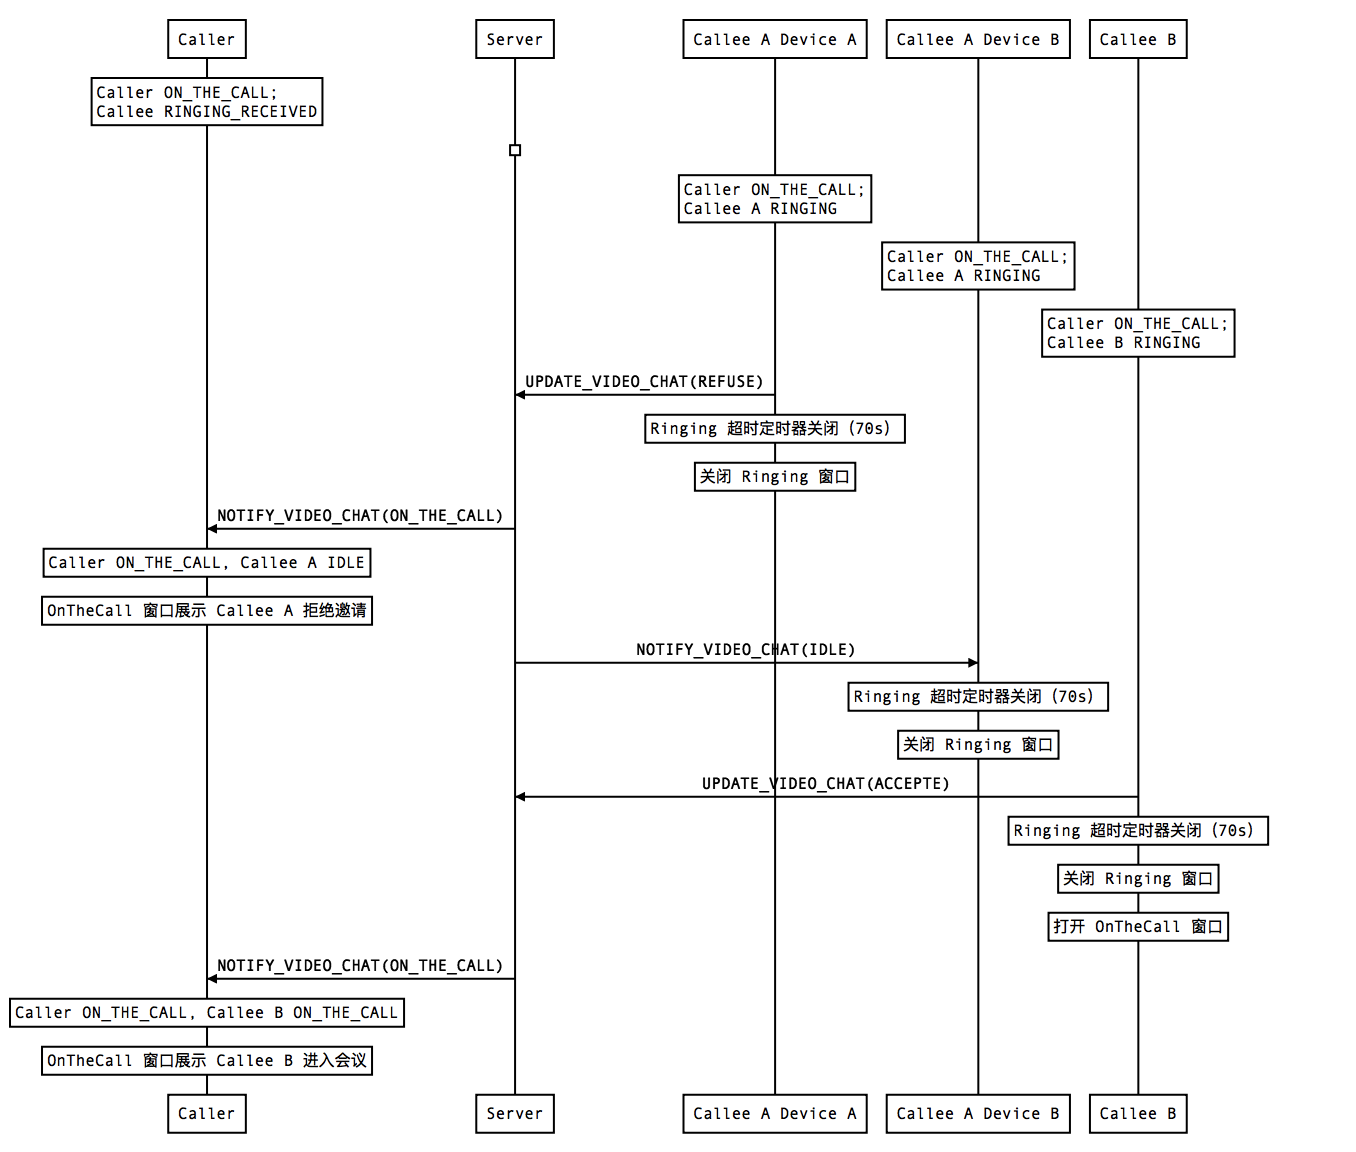
\includegraphics{/Users/billchen/Workspace/LearningRepo/Course/SoftwareRequirements/Yoom/Sequence Diagram/07_nvn_accept_invitation.png}
\caption{}
\end{figure}

\texttt{YM1002-SQ04:\ nvn\_refuse\_invitation}:NvN 拒绝通话邀请:

\begin{figure}
\centering
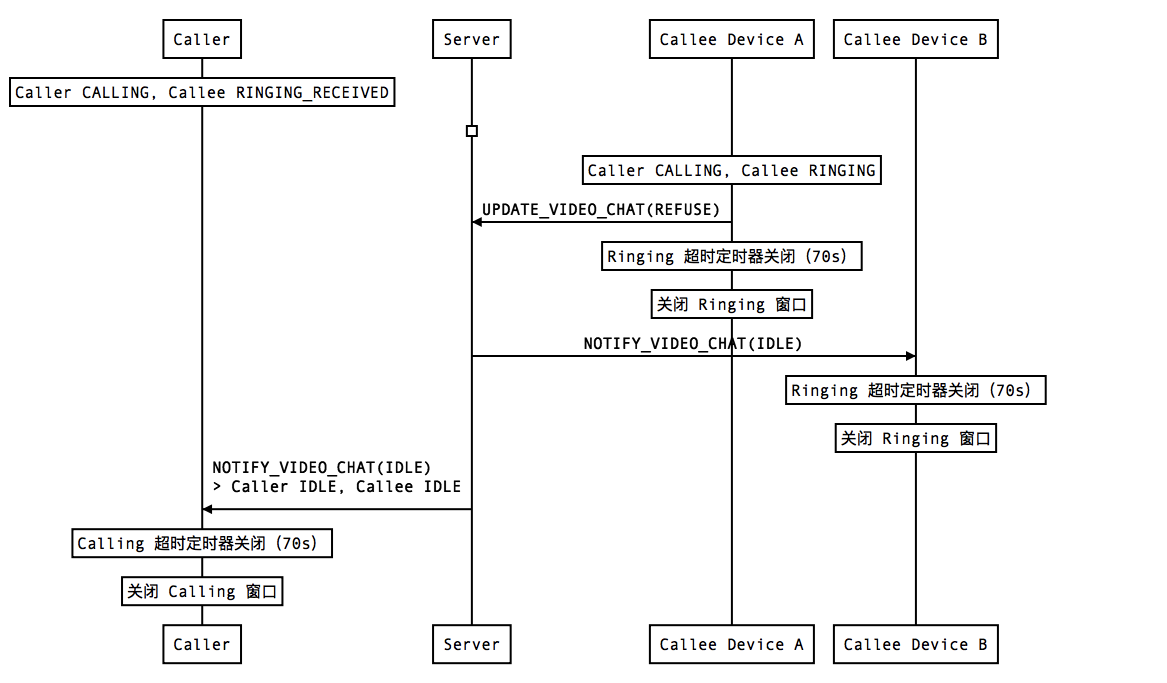
\includegraphics{/Users/billchen/Workspace/LearningRepo/Course/SoftwareRequirements/Yoom/Sequence Diagram/08_nvn_refuse_invitation.png}
\caption{}
\end{figure}

\texttt{YM1002-SQ04:\ nvn\_refuse\_invitation}:NvN
通话主持人离开会议,并移交主持人权限:

\begin{figure}
\centering
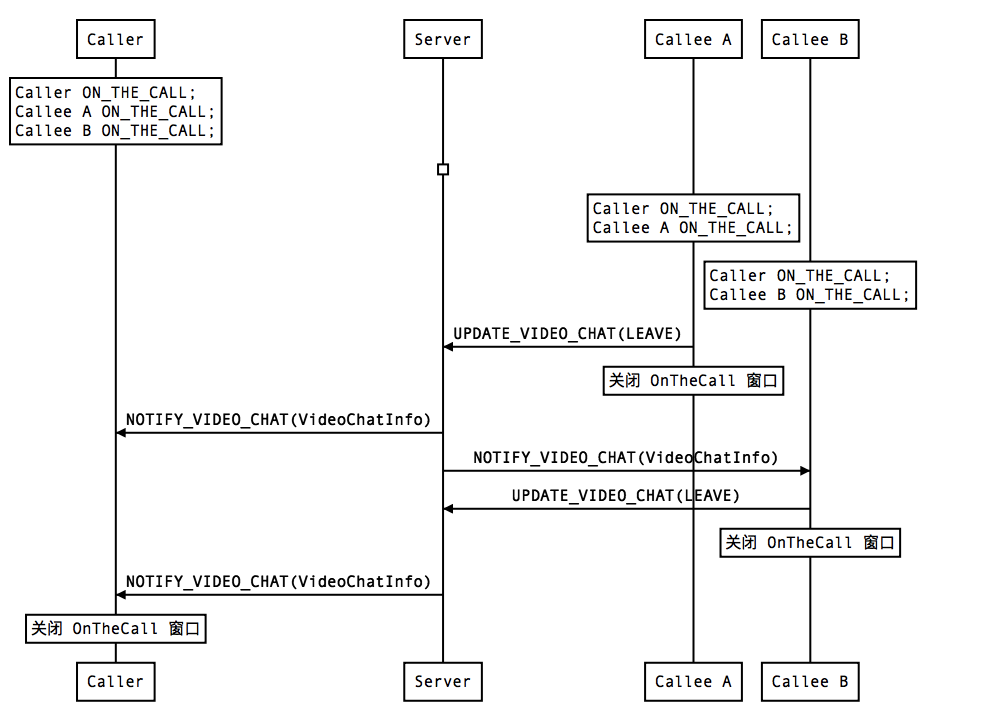
\includegraphics{/Users/billchen/Workspace/LearningRepo/Course/SoftwareRequirements/Yoom/Sequence Diagram/09_nvn_leave_meeting.png}
\caption{}
\end{figure}

\texttt{YM1002-SQ04:\ nvn\_refuse\_invitation}:NvN
通话结束会议,并解散所有参会者:

\begin{figure}
\centering
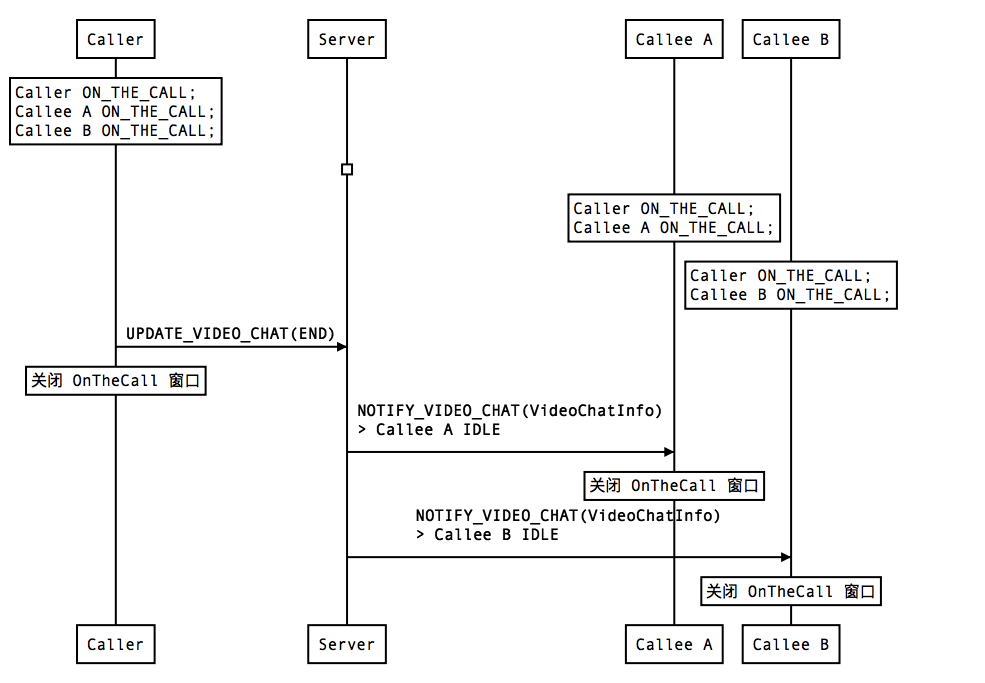
\includegraphics{/Users/billchen/Workspace/LearningRepo/Course/SoftwareRequirements/Yoom/Sequence Diagram/10_nvn_end_meeting.png}
\caption{}
\end{figure}

\hypertarget{ux9700ux6c42ux63cfux8ff0ux53caux7528ux4f8bux63cfux8ff0-2}{%
\paragraph{需求描述及用例描述}\label{ux9700ux6c42ux63cfux8ff0ux53caux7528ux4f8bux63cfux8ff0-2}}

\begin{itemize}
\item
  NVN
\end{itemize}

该需求涉及到的主要用例有 Join Meeting By PSTN, Join Meeting By Meeting
ID, Join Meeting by Meeting Link

\hypertarget{ux7528ux4f8bux63cfux8ff0join-meeting-by-link}{%
\subparagraph{用例描述:Join Meeting By
Link}\label{ux7528ux4f8bux63cfux8ff0join-meeting-by-link}}

\begin{longtable}[]{@{}ll@{}}
\toprule
Key & Value\tabularnewline
\midrule
\endhead
Use Case & Join Meeting By Link\tabularnewline
Actors & Non-participant, Host\tabularnewline
Pre-condition &
\vtop{\hbox{\strut 用户应当正确登录进了系统;}\hbox{\strut Non-participant
拥有了 1v1 通话的邀请链接}}\tabularnewline
Post-condition & Non-participant 被 Host 邀请进该会议\tabularnewline
Main Flow & Non-participant 打开链接,进入会议\tabularnewline
Alternative Flow & \vtop{\hbox{\strut Non-participant
当前正在另一个会议,并打开了链接:}\hbox{\strut Non-participant
选择是否接受会议邀请,如果接受邀请,则退出当前会议,并加入新的会议}\hbox{\strut 如果拒接邀请,则忽略该邀请,用户继续在原会议进行通话}\hbox{\strut 该会议设置了入会权限,需要在等候室确认主持人进入会议系统之后再}}\tabularnewline
Exception & None\tabularnewline
\bottomrule
\end{longtable}

\hypertarget{ym2001ux4f1aux4e2dux53c2ux4f1aux6743ux9650ux7ba1ux7406}{%
\subsubsection{YM2001:会中参会权限管理}\label{ym2001ux4f1aux4e2dux53c2ux4f1aux6743ux9650ux7ba1ux7406}}

\hypertarget{ux7528ux6237ux754cux9762-3}{%
\paragraph{用户界面}\label{ux7528ux6237ux754cux9762-3}}

\hypertarget{ux9700ux6c42ux63cfux8ff0ux53caux7528ux4f8bux63cfux8ff0-3}{%
\paragraph{需求描述及用例描述}\label{ux9700ux6c42ux63cfux8ff0ux53caux7528ux4f8bux63cfux8ff0-3}}

\hypertarget{ym3001ux5b9eux65f6ux5b57ux5e55}{%
\subsubsection{YM3001:实时字幕}\label{ym3001ux5b9eux65f6ux5b57ux5e55}}

\hypertarget{ux7528ux6237ux754cux9762-4}{%
\paragraph{用户界面}\label{ux7528ux6237ux754cux9762-4}}

\hypertarget{ux9700ux6c42ux63cfux8ff0ux53caux7528ux4f8bux63cfux8ff0-4}{%
\paragraph{需求描述及用例描述}\label{ux9700ux6c42ux63cfux8ff0ux53caux7528ux4f8bux63cfux8ff0-4}}

\begin{itemize}
\item
  需要在会中
\item
  主持人 Host 和联席主持人 Co-Host
\end{itemize}

\hypertarget{ym3002ux4f1aux4e2dux7279ux6548}{%
\subsubsection{YM3002:会中特效}\label{ym3002ux4f1aux4e2dux7279ux6548}}

\hypertarget{ux7528ux6237ux754cux9762-5}{%
\paragraph{用户界面}\label{ux7528ux6237ux754cux9762-5}}

\hypertarget{ux9700ux6c42ux63cfux8ff0ux53caux7528ux4f8bux63cfux8ff0-5}{%
\paragraph{需求描述及用例描述}\label{ux9700ux6c42ux63cfux8ff0ux53caux7528ux4f8bux63cfux8ff0-5}}

\hypertarget{ux6027ux80fdux9700ux6c42--performace-requirements}{%
\subsection{性能需求 / Performace
Requirements}\label{ux6027ux80fdux9700ux6c42--performace-requirements}}

\hypertarget{ym10011v1-ux901aux8bdd-2}{%
\subsubsection{YM1001:1v1 通话}\label{ym10011v1-ux901aux8bdd-2}}

\hypertarget{ym1002nvn-ux901aux8bdd-2}{%
\subsubsection{YM1002:NvN 通话}\label{ym1002nvn-ux901aux8bdd-2}}

\hypertarget{ux5916ux90e8ux7cfbux7edfux9650ux5236--design-constraints}{%
\subsection{外部系统限制 / Design
Constraints}\label{ux5916ux90e8ux7cfbux7edfux9650ux5236--design-constraints}}

\hypertarget{ux7ec8ux7aefux5e73ux53f0ux8981ux6c42}{%
\subsubsection{终端平台要求}\label{ux7ec8ux7aefux5e73ux53f0ux8981ux6c42}}

\hypertarget{ux79fbux52a8ux7aef}{%
\paragraph{移动端}\label{ux79fbux52a8ux7aef}}

Yoom Meetings 安卓端最低适配到基于 Android 5.0
的设备,手机的分辨率不应低于 720x1080。最低的内存配置为
2GB,推荐的内存配置为 3GB 及以上。

iOS 端支持在 iOS 12.0 及以上的系统的所有苹果设备,包括:

\begin{longtable}[]{@{}lll@{}}
\toprule
iPad & iPhone & Apple Watch\tabularnewline
\midrule
\endhead
iPad & &\tabularnewline
\bottomrule
\end{longtable}

PS. 暂时不兼容使用鸿蒙系统的华为终端手机设备,预计在 2021
年第四季度完成适配工作。

\hypertarget{ux684cux9762ux7aef}{%
\paragraph{桌面端}\label{ux684cux9762ux7aef}}

Yoom Meetings 的 Windows 端可在 Windows 7
及更高版本的系统上运行。目前已在 Windows 10 20H2
版本上测试通过,无运行异常。

最低配置要求:

\begin{itemize}
\item
  Intel Corel i3
\item
  4GB 运行内存
\item
  1280 x 720 分辨率
\end{itemize}

推荐配置要求:

\begin{itemize}
\item
  Intel Corel i3
\item
  8GB 运行内存
\item
  1280 x 720 屏幕分辨率
\end{itemize}

mac 端目前兼容了 macOS 10.11 及更高级的版本,在苹果 2014
年及之后发布的设备中可用。

\hypertarget{ux7f51ux9875ux7aef}{%
\paragraph{网页端}\label{ux7f51ux9875ux7aef}}

受限于浏览器 API 限制,Yoom Meetings 应当在以下浏览器上运行

\begin{longtable}[]{@{}llllllll@{}}
\toprule
系统 & Chrome & Firefox & Safari & Edge & Edge Chromium & Internet
Explorer & Opera\tabularnewline
\midrule
\endhead
Windows & √ & √ & - & √ & √ & × & √\tabularnewline
Android & √ & √ & - & - & √ & - & √\tabularnewline
iOS & √ & √ & √* & - & √ & - & √\tabularnewline
macOS & √ & √ & √* & - & √ & - & √\tabularnewline
Linux & √ & √ & - & - & - & - & √\tabularnewline
\bottomrule
\end{longtable}

注:在使用 Yoom Meetings
之前,请将浏览器升级至最新版本。以上兼容性报告均在截止 2021 年 6 月 15
日前的最新版本上测试。

*:会中特效功能暂时无法在 Safari 浏览器上使用。

\hypertarget{ux786cux4ef6ux8981ux6c42}{%
\subsubsection{硬件要求}\label{ux786cux4ef6ux8981ux6c42}}

\hypertarget{ux7f51ux7edcux4e0aux884cux5e26ux5bbdux8981ux6c42}{%
\paragraph{网络上行带宽要求}\label{ux7f51ux7edcux4e0aux884cux5e26ux5bbdux8981ux6c42}}

为了保证会议质量,使用 Yoom Meetings
系统的网络上行带宽需要满足下列需求:

\begin{longtable}[]{@{}lll@{}}
\toprule
场景 & 终端 & 带宽要求\tabularnewline
\midrule
\endhead
音频会议 & 移动端/桌面端/网页端 & 64 Kbps\tabularnewline
视频会议 & 移动端 & 1 Mbps (高质量视频)\tabularnewline
视频会议 & 桌面端 & 3 Mbps (高质量视频)\tabularnewline
视频会议 & 网页端 & 2 Mbps (高质量视频)\tabularnewline
屏幕共享 & 移动端/桌面端/网页端 & 2 Mbps (高质量屏幕)\tabularnewline
\bottomrule
\end{longtable}

备注:各终端在网络条件受限的情况下,Yoom 会自动调整带宽至 0.5 Mbps。

\hypertarget{ux7f51ux7edcux4e0bux884cux5e26ux5bbdux8981ux6c42}{%
\paragraph{网络下行带宽要求}\label{ux7f51ux7edcux4e0bux884cux5e26ux5bbdux8981ux6c42}}

为了保证会议质量,使用 Yoom Meetings
系统的网络下行带宽需要满足下列需求:

\begin{longtable}[]{@{}lll@{}}
\toprule
场景 & 终端 & 带宽要求\tabularnewline
\midrule
\endhead
音频会议 & 移动端/桌面端/网页端 & 192 Kbps\tabularnewline
视频会议 - 宫格视图 & 移动端 & 0.5 Mbps (高质量视频)\tabularnewline
视频会议 - 缩略视图 & 移动端 & 0.5 Mbps (高质量视频)\tabularnewline
视频会议 - 宫格视图 & 桌面端 & 1 Mbps (高质量视频)\tabularnewline
视频会议 - 缩略视图 & 桌面端 & 2 Mbps (高质量视频)\tabularnewline
视频会议 - 演讲者视图 & 桌面端 & 3 Mbps (高质量视频)\tabularnewline
视频会议 - 宫格视图 & 网页端 & 1 Mbps (高质量视频)\tabularnewline
视频会议 - 缩略视图 & 网页端 & 2 Mbps (高质量视频)\tabularnewline
视频会议 - 演讲者视图 & 网页端 & 3 Mbps (高质量视频)\tabularnewline
\bottomrule
\end{longtable}

备注:以上带宽要求为实现单流推送的最低网络要求,如要实现更高质量的会议或支持千方会议,需要将各项的带宽需求提升
3 倍,否则可能会出现性能问题或卡顿。


\hypertarget{ux9644ux5f55--appendix}{%
\subsection{附录 / Appendix}\label{ux9644ux5f55--appendix}}

\hypertarget{ux4feeux8ba2ux8bb0ux5f55--version-records}{%
\subsubsection{修订记录 / Version
Records}\label{ux4feeux8ba2ux8bb0ux5f55--version-records}}

\hypertarget{v02}{%
\subsubsection{V0.2}\label{v02}}

\hypertarget{v01}{%
\subsubsection{V0.1}\label{v01}}

\begin{longtable}[]{@{}ll@{}}
\toprule
Key & Value\tabularnewline
\midrule
\endhead
版本号 & 0.1\tabularnewline
修订日期 & 2021-06-01\tabularnewline
修订内容 & 初始版本发布\tabularnewline
需求影响 & 无\tabularnewline
评审人 & @William Tester, @Charlie Tester\tabularnewline
评审日期 & 2021-06-02\tabularnewline
评审结果 & 通过\tabularnewline
文件存档 &
\url{https://example.com/yoommeetings/sds0.1.pdf}\tabularnewline
\bottomrule
\end{longtable}


本需求文档基于在实习期间接触到的真实商业项目完成,出于商业保密要求,需求文档具体参数内容、系统名称等内容为合理范围内的的虚构,仅供满足课程考核需求。

陈俊潼 · 2021 年 6 月

华东师范大学 · 软件工程学院

\end{document}
